\documentclass[24pt,a4paper]{article}% 文档格式
\usepackage{ctex,hyperref}% 输出汉字
\usepackage{times}% 英文使用Times New Roman
%%%%%%%%%%%%%%%%%%%%%%%%%%%%%%%%%%%%%%%%%%%%%%%%%%%%%%%%
\title{\fontsize{18pt}{27pt}\selectfont% 小四字号,1.5倍行距
	{\heiti% 黑体 
		一种\LaTeX 模板}}% 题目
%%%%%%%%%%%%%%%%%%%%%%%%%%%%%%%%%%%%%%%%%%%%%%%%%%%%%%%%
\date{}% 日期(这里避免生成日期)
%%%%%%%%%%%%%%%%%%%%%%%%%%%%%%%%%%%%%%%%%%%%%%%%%%%%%%%%
\usepackage{amsmath,amsfonts,amssymb}% 为公式输入创造条件的宏包
%%%%%%%%%%%%%%%%%%%%%%%%%%%%%%%%%%%%%%%%%%%%%%%%%%%%%%%%
\usepackage{graphicx}% 图片插入宏包
\usepackage{subfigure}% 并排子图
\usepackage{float}% 浮动环境,用于调整图片位置
\usepackage[export]{adjustbox}% 防止过宽的图片
\usepackage{caption}
%%%%%%%%%%%%%%%%%%%%%%%%%%%%%%%%%%%%%%%%%%%%%%%%%%%%%%%%
\usepackage{url}% 超链接
\usepackage{bm}% 加粗部分公式
\usepackage{multirow}
\usepackage{booktabs}
\usepackage{epstopdf}
\usepackage{epsfig}
\usepackage{longtable}% 长表格
\usepackage{supertabular}% 跨页表格
\usepackage{algorithm}
\usepackage{algorithmic}
\usepackage{changepage}% 换页
\usepackage{listings}% 插入代码段
%%%%%%%%%%%%%%%%%%%%%%%%%%%%%%%%%%%%%%%%%%%%%%%%%%%%%%%%
\usepackage[left=2.50cm,right=2.50cm,top=2.80cm,bottom=2.50cm]{geometry}% 页边距设置
\renewcommand{\baselinestretch}{1.5}% 定义行间距(1.5)
\renewcommand{\contentsname}{\normalfont \kaishu \Huge 目录}% 定义目录两字的格式

\usepackage{subfigure}% 有关设置目录引导点的宏包
\usepackage[subfigure]{tocloft}
\renewcommand{\cftsecleader}{\cftdotfill{\cftdotsep}} % 给 sections加点
\newcommand\mydot[1]{\scalebox{#1}{.}}
\renewcommand\cftdot{\mydot{0.8}} % change the size of dots
\renewcommand\cftdotsep{3} % change the space between dots

\hypersetup{
colorlinks=true,
linkcolor=black
}% 设置链接的颜色,防止目录出现红框
%%%%%%%%%%%%%%%%%%%%%%%%%%%%%%%%%%%%%%%%%%%%%%%%%%%%%%%%

\begin{document}% 以下为正文内容
\begin{titlepage}
    \centering
    
\includegraphics[width=0.3\textwidth]{image/zju_logo.png}\par\vspace{5cm}
    {\huge\songti 需求分析报告\par}
    \vspace{1cm}
    {\Large\itshape 第三大组第三小组\par}
    \vspace{7cm}
    \vfill
    {\large \today\par}
\end{titlepage}
\newpage

\begin{center}
    \kaishu
    \tableofcontents
    \setcounter{page}{0}
    \thispagestyle{empty} % 设置目录页的页脚为空
\end{center}
\newpage

\section*{\songti 第一部分:引言}
\addcontentsline{toc}{section}{1.引言}
\subsection*{\songti 1.1编写目的}
\addcontentsline{toc}{subsection}{1.1编写目的}
随着移动互联网、人工智能、大数据等技术快速发展,越来越多的人享受到互联网医疗带来的便利服务。例如,在线开具电子处方,药品直接快递到家;远程诊疗,在乡镇医院也能享受省级专家会诊;开通电子社保卡,动动手指就能挂号缴费。互联网医疗借助防疫期间庞大的用户需求,实现迅猛发展,并不断向潜在用户渗透。我们希望编写一个综合性的互联网在线医疗平台,为病人、医生和院方提供流程和管理上的便利。
\subsection*{\songti 1.2相关背景}
\addcontentsline{toc}{subsection}{1.2相关背景}
该项目开发的软件为一个综合性的互联网在线医疗平台,旨在为病人、医生和院方提供便利的医疗服务。
该平台将采用前后端分离的架构,前端使用Vue3框架实现用户界面,后端使用Spring Boot框架开发服务器端逻辑,数据库采用MySQL关系型数据库。
相较于传统的“纸质+线下”模式而言,该项目的“互联网+”医疗模式具有便于归档的优势,并且可以使得医疗资源匮乏的地区也能享受到高质量的医疗服务。
该平台将整合医院的资源,提供在线挂号、预约、缴费、问诊等服务,让病人、医生和管理人员足不出户便能完成全过程的在线问诊。
该平台将采用多种信息安全技术保护用户信息和交易安全。
该平台将遵循便民、利民的理念,简化操作流程、美化操作界面、便利各方用户的使用。 \par
平台上线后,病人可以通过平台进行挂号、预约、缴费、问诊等操作,医生可以通过平台进行打卡、上班、请假、查询等操作,管理人员可以通过平台进行药房管理、医生管理、病人管理、投诉管理等操作。 \par
本小组负责开发的子系统实现了线上问诊与投诉功能,以及管理端的投诉处理功能。
\newpage
\subsection*{\songti 1.3定义部分}
\addcontentsline{toc}{subsection}{1.3定义部分}
\subsubsection*{\songti 1.3.1\ Linux}
Linux是一种自由和开放源码的类UNIX操作系统。该操作系统的内核由Linus·Torvalds在1991年10月5日首次发布。Ubuntu 22.04 LTS是Canonical于2022年4月21日发布的Linux发行版之一。本项目运行在云端Ubuntu操作系统的服务器上。
\subsubsection*{\songti 1.3.2\ MySql}
MySQL是一个关系型数据库管理系统,由瑞典MySQL AB公司开发,属于Oracle旗下产品。MySQL是最流行的关系型数据库管理系统之一,在WEB应用方面,MySQL是最好的RDBMS应用软件之一。本项目采用MySQL作为数据库管理系统。
\subsubsection*{\songti 1.3.3\ SpringBoot}
Spring Boot是由Pivotal团队提供的全新框架,其设计目的是用来简化新Spring应用的初始搭建以及开发过程。该框架使用了特定的方式来进行配置,从而使开发人员不再需要定义样板化的配置。本项目采用Spring Boot作为后端开发的框架。
\subsubsection*{\songti 1.3.4\ Vue3}
Vue是一款用于构建用户界面的JavaScript框架。它基于标准HTML、CSS 和JavaScript构建,并提供了一套声明式的、组件化的编程模型,帮助你高效地开发用户界面。无论是简单还是复杂的界面,Vue都可以胜任。本项目采用Vue3作为前端开发的框架。
\subsubsection*{\songti 1.3.5\ 用例}
用例(use case),是软件工程或系统工程中对系统如何反应外界请求的描述,是一种通过用户的使用场景来获取需求的技术。每个用例提供了一个或多个场景,该场景说明了系统是如何和最终用户或其它系统互动,也就是谁可以用系统做什么,从而获得一个明确的业务目标。
\subsubsection*{\songti 1.3.6\ 用例图}
用例图(use case diagram)是用户与系统交互的最简表示形式,展现了用户和与他相关的用例之间的关系。通过用例图,人们可以获知系统不同种类的用户和用例。用例图也经常和其他图表配合使用。\par
用例图的目的就是为了可以让人在一个更高的层次概览整个系统,用平白的话语让项目参与者理解系统。它可以辅以额外的图表和文档,以更加完整地展现系统的功能和技术细节。
\subsubsection*{\songti 1.3.7\ 状态图}
状态图(Statechart Diagram)是UML的五个图之一,用来模拟系统的动态性质。它们定义了一个对象在其生命周期中的不同状态,这些状态由事件改变。状态图对于建模反应式系统很有用。反应式系统可以被定义为对外部或内部事件做出反应的系统。\par
状态图描述了从一个状态到另一个状态的控制流。状态被定义为一个对象存在的条件,当一些事件被触发时,它就会改变。状态图最重要的目的是对一个对象从创建到终止的生命周期进行建模。
\subsubsection*{\songti 1.3.8\ 数据流图}
数据流图(Data Flow Diagram)是描述系统中数据流程的一种图形工具,它标志了一个系统的逻辑输入和逻辑输出,以及把逻辑输入转换逻辑输出所需的加工处理。\par
数据流图不是传统的流程图或框图,数据流也不是控制流。数据流图是从数据的角度来描述一个系统,而框图是从对数据进行加工的工作人员的角度来描述系统。
\subsubsection*{\songti 1.3.9\ CRC卡}
CRC卡(Class-Responsibility-Collaborator)是一种在面向对象分析建模中常用的工具。这个方法在面向对象工程设计中非常流行。用户、设计者和开发人员都参与其中,完成对整个面向对象系统的设计。它包括三个部分:类名、类的职责和类的协作。CRC卡是一个标准索引卡集合,每张卡片表示一个类。这种方法帮助我们更好地理解系统的结构,确保设计的高质量和可维护性。
\subsubsection*{\songti 1.3.10\ 类图}
类图(Class diagram)是软件工程的统一建模语言一种静态结构图,该图描述了系统的类集合,类的属性和类之间的关系。类图是面向对象式的建模。他们一般都被用于概念建模(conceptual modelling)的系统分类的应用程序,并可将模型建模转译成代码。

% \begin{thebibliography}{99}
%     \bibitem{ref1} 到底什么是智慧医疗?.知乎.\url{https://zhuanlan.zhihu.com/p/370146544}
%     \bibitem{ref2} 电子处方、远程诊疗、手机缴费——在线服务让病人少跑医院.人民日报海外版.\url{https://www.gov.cn/xinwen/2022-03/11/content_5678414.htm}
%     \addcontentsline{toc}{subsection}{1.4参考文献} %向目录中添加条目,以章的名义
% \end{thebibliography}
\newpage

\section*{\songti 第二部分:任务概述}
\addcontentsline{toc}{section}{2.任务概述}
\subsection*{\songti 2.1系统概述}
\addcontentsline{toc}{subsection}{2.1系统概述}
本小组负责的问诊投诉子系统是整个医疗系统的一个重要组成部分,提供了病人和医生之间的在线问诊服务,以及病人对医生和医院的投诉功能。
医生与病人可以通过系统进行在线问诊,病人可以向医生咨询病情、诊断结果、治疗方案等问题,医生可以根据病人的症状和病史进行诊断和治疗建议。
同时,病人还可以对医生和医院的服务进行评价和投诉,以提高医疗服务的质量和效率。
问诊投诉子系统的目标是提供便捷、高效、安全的在线问诊服务,为病人和医生提供更好的医疗体验。
\subsection*{\songti 2.2系统组成}
\addcontentsline{toc}{subsection}{2.2系统组成}
本系统的架构包括前端界面、后端服务器和数据库:\par \noindent 前端界面:用户通过Web页面或移动应用程序与系统进行交互。\par \noindent 后端服务器:包括用户管理、医生管理等模块,处理用户请求并与数据库交互。\par \noindent 数据库:存储用户信息、医疗记录和系统配置等数据。\par
技术实现:系统采用前后端分离的架构,前端使用HTML、CSS和JavaScript并采取Vue3框架实现用户界面,后端使用Java语言和SpringBoot框架开发服务器端逻辑,数据库采用MySQL关系型或非关系型数据库。同时采取诸如AES,SHA-1等加密算法保护用户数据安全。
\subsection*{\songti 2.3用户特点}
\addcontentsline{toc}{subsection}{2.3用户特点}
病人用户:寻求医疗帮助的个人,他们可能是有健康问题或需要医疗咨询的患者。他们可能更愿意在舒适的家中或办公室环境下就诊,而不是前往医院或诊所。医生用户:注册在系统中提供医疗服务的专业医生和医护人员。具有丰富的医疗知识和经验,可以为病人提供诊断、治疗建议和处方。管理员用户:负责管理药房,同时掌控病人、医生和医院的所有信息。需要监督系统的安全性和稳定性,确保用户数据的保密性和完整性。
\subsection*{\songti 2.4假定和约束}
\addcontentsline{toc}{subsection}{2.4假定和约束}
1.本系统假定,背景是在一个物联网高度发达的环境下。\par
2.本系统假定三方使用者都是在家然后线上在线完成全过程的。\par
3.本系统假定结果是全国的医疗系统都共同可以查询的。\par
4.本系统假定药品采用邮寄的形式寄送到家中。\par
5.本系统假定病人一天内的所有活动同属一张病历单,不存在一天看两种不同病的可能性。\par
6.本系统规定病人第一天和第二天的看病不属于一张病历单。
\newpage

\section*{\songti 第三部分:需求规定}
\addcontentsline{toc}{section}{3.需求规定}
\subsection*{\songti 3.1功能要求}
\addcontentsline{toc}{subsection}{3.1功能要求}
\noindent (1)基本功能:系统能够执行其基本预期的功能,满足用户最基本的需求。 \par
\noindent (2)数据处理功能:系统能够有效地处理用户输入的数据,并根据需要进行存储、检索、修改和删除等操作。数据处理功能应该准确、可靠,并保证数据的完整性和安全性。\par
\noindent (3)安全功能:系统应该具有必要的安全功能,包括身份认证、权限控制、数据加密等。系统应该能够防范各种安全威胁,如SQL注入、跨站脚本攻击等。\par
\noindent (4)可扩展性功能:系统应该具有良好的可扩展性,能够方便地进行功能扩展和模块添加。系统应该支持插件化或模块化的设计,以便将来根据需要进行功能的增加和修改。\par
\noindent (5)可维护性功能:系统应该易于维护和管理,包括代码结构清晰、注释充分、文档完备等。系统应该具有良好的可读性和可维护性,便于开发团队进行后续的维护和修改。
\subsection*{\songti 3.2性能要求}
\addcontentsline{toc}{subsection}{3.2性能要求}
\noindent (1)响应时间要求:\par 系统对用户请求的响应时间要求,在用户发起请求后系统应尽快返回结果,以保证用户体验。\par
\noindent (2)吞吐量要求:\par 系统应在单位时间内能够处理的请求或事务数量的要求,通常用于衡量系统的处理能力。\par
\noindent (3)并发性能要求:\par 系统应能够同时处理的用户数量或并发请求数量的要求,涉及系统的并发处理能力。\par
\noindent (4)容错性能要求:\par 系统应在出现性能问题或部分故障时有容错处理能力,保障系统的稳定性和可靠性。\par
\noindent (5)资源利用效率要求:\par 系统应能有效地利用计算资源、存储资源和网络带宽,以提高系统的性能。\par
\noindent (6)可用时间性能要求:\par 系统应有可用时间性能要求,即系统在一定时间内可用的比例,通常以百分比表示。\par
\subsection*{\songti 3.3接口要求}
\addcontentsline{toc}{subsection}{3.3接口要求}
首先,接口应该被清晰地定义和文档化,包括输入参数、输出参数、返回值类型、异常处理等内容,以便开发人员正确地使用接口。其次,接口应该保证稳定性、一致性、安全性、可用性,同时易于使用和理解,具有良好的可读性和可维护性。其次,接口应该具有良好的扩展性和兼容性,能够方便地进行功能扩展和接口升级。最后,接口应该具有良好的性能和效率,能够快速响应用户请求,保证系统的高性能和高可用性。
\subsection*{\songti 3.4界面要求}
\addcontentsline{toc}{subsection}{3.4界面要求}
首先,界面应该设计得简洁明了,易于理解和操作。同时,使用直观的图标、文字和布局,提供统一的视觉风格和操作方式。界面应该具有良好的响应性,快速响应用户的操作,且能够友好地处理用户输入错误或操作失误。加之提供及时的交互反馈,如动画效果、进度条等。
\newpage

\section*{\songti 第四部分:用户场景}
\addcontentsline{toc}{section}{4.用户场景}
\addcontentsline{toc}{subsection}{4.0总体框架介绍}
\begin{figure}[H]
    \centering
    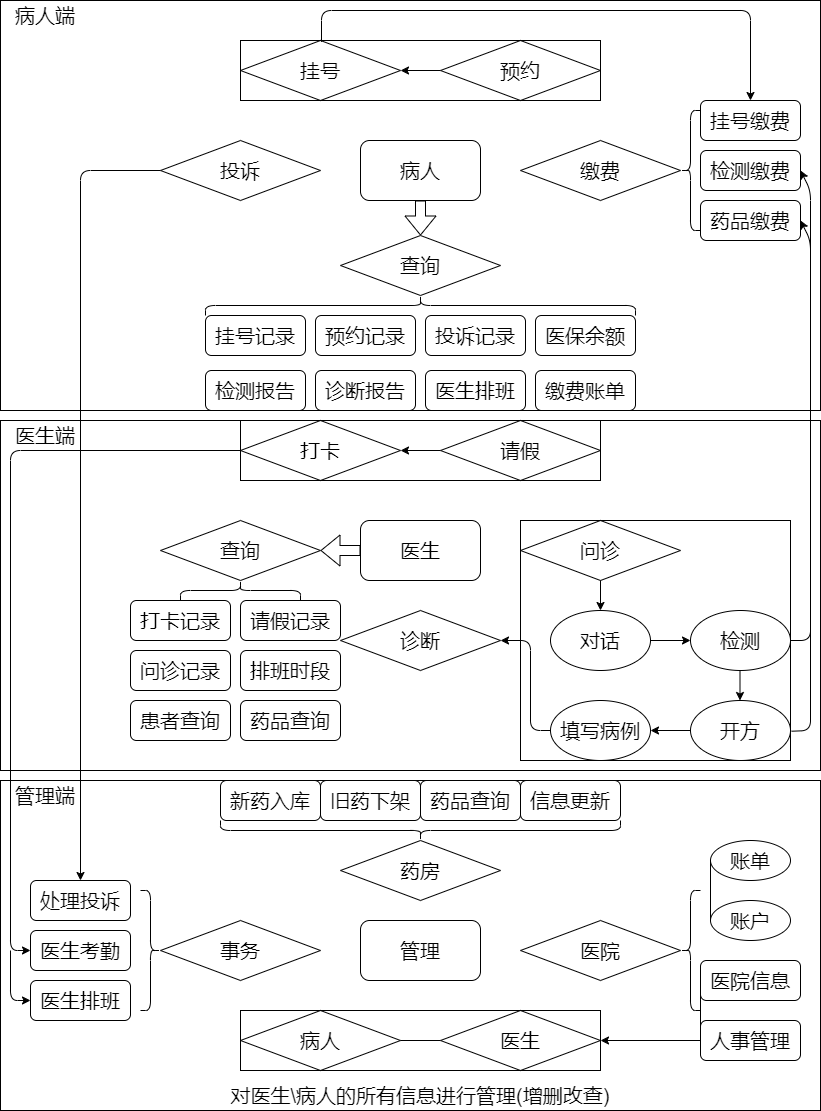
\includegraphics[width=1\textwidth]{image/architecture.png}
    \caption*{图1.总架构图}
\end{figure}
\begin{figure}[H]
    \centering
    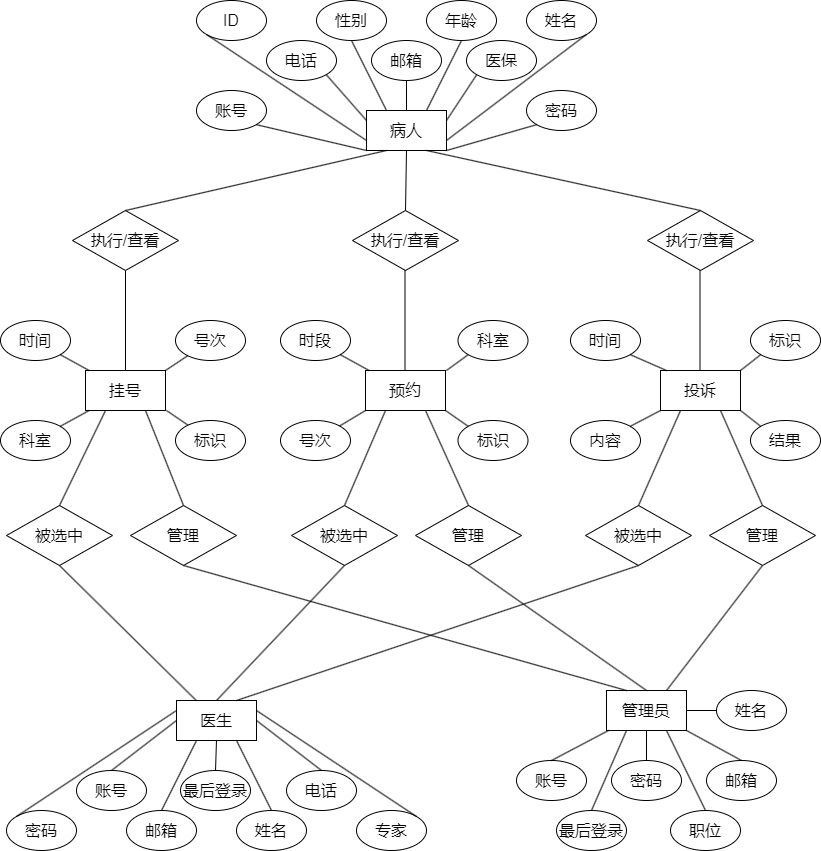
\includegraphics[width=1\textwidth]{image/ERGraph1.png}
    \caption*{图2.E-R图(1)}
\end{figure}
这张是病人的一些基础功能的E-R图,包括挂号、预约和投诉与各个实体之间的关系。
\begin{figure}[H]
    \centering
    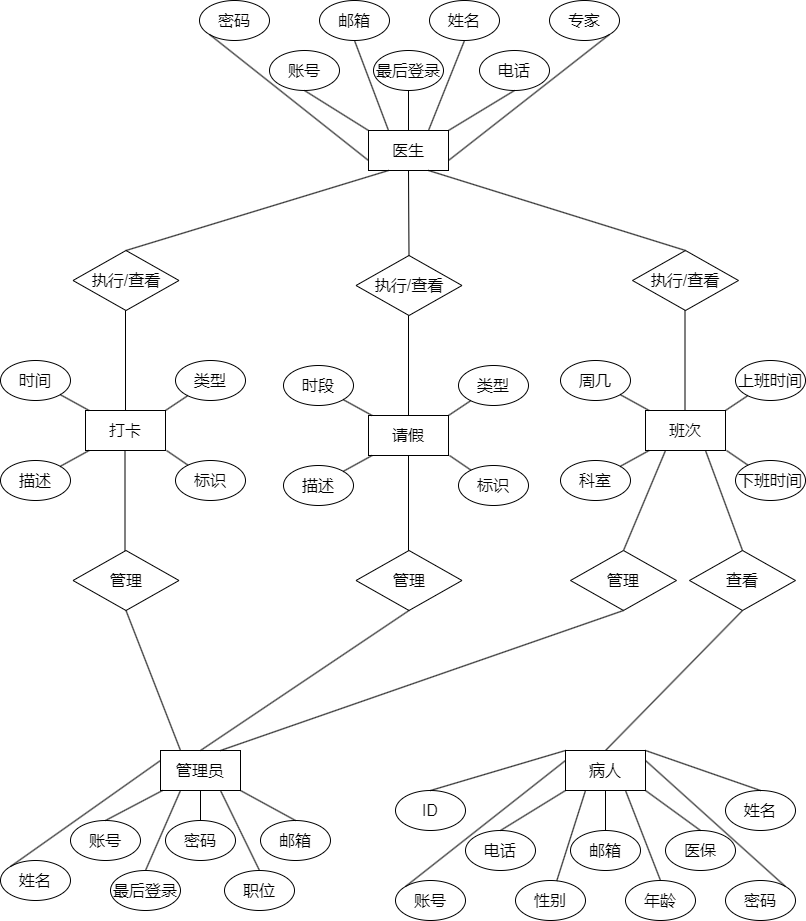
\includegraphics[width=1\textwidth]{image/ERGraph2.png}
    \caption*{图3.E-R图(2)}
\end{figure}
这张是医生的一些基础功能的E-R图,包括打卡、请假和排班与各个实体之间的关系。
\begin{figure}[H]
    \centering
    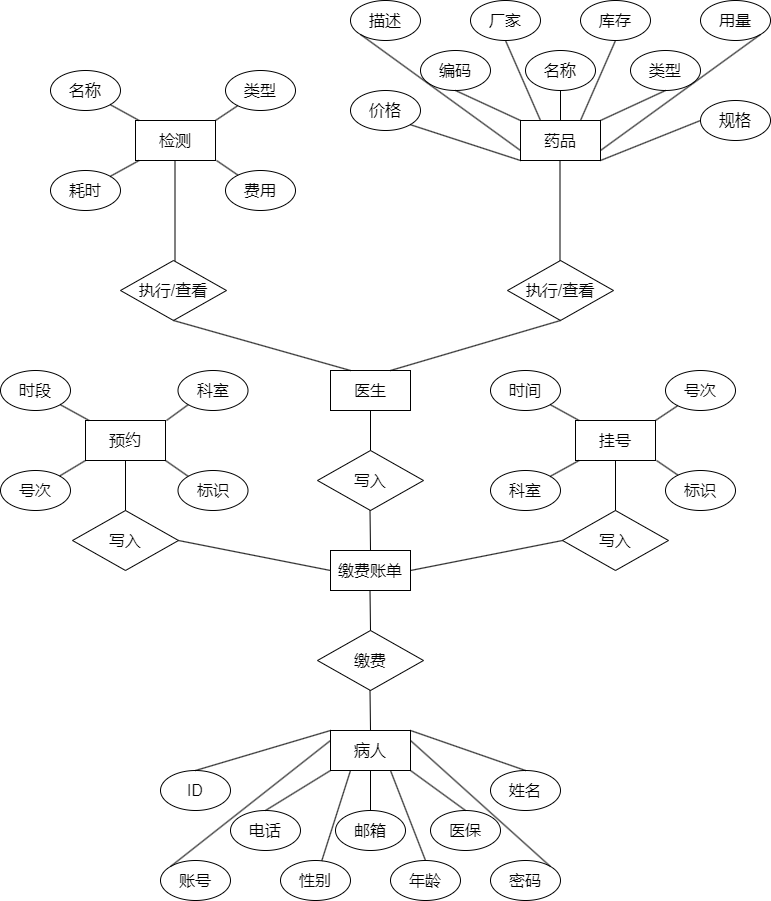
\includegraphics[width=1\textwidth]{image/ERGraph3.png}
    \caption*{图4.E-R图(3)}
\end{figure}
这张是用来描述医生与检测和开方以及病人与缴费各个实体之间关系的E-R图。
\begin{figure}[H]
    \centering
    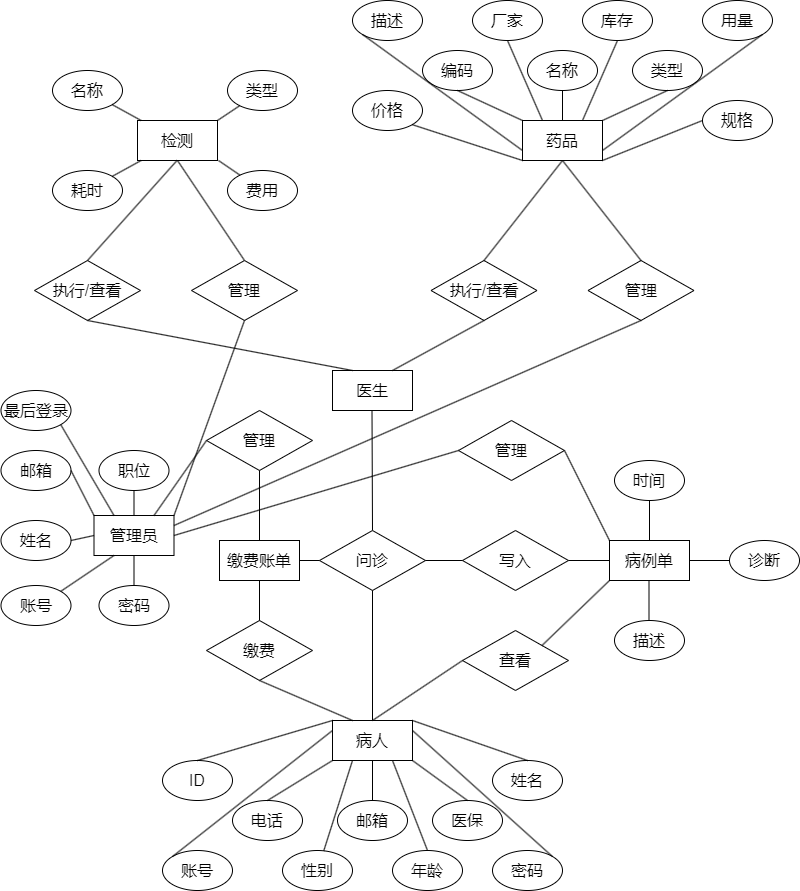
\includegraphics[width=1\textwidth]{image/ERGraph4.png}
    \caption*{图5.E-R图(4)}
\end{figure}
这张是用来重点描述病人医生问诊时各个实体之间关系的E-R图。
\begin{figure}[H]
    \centering
    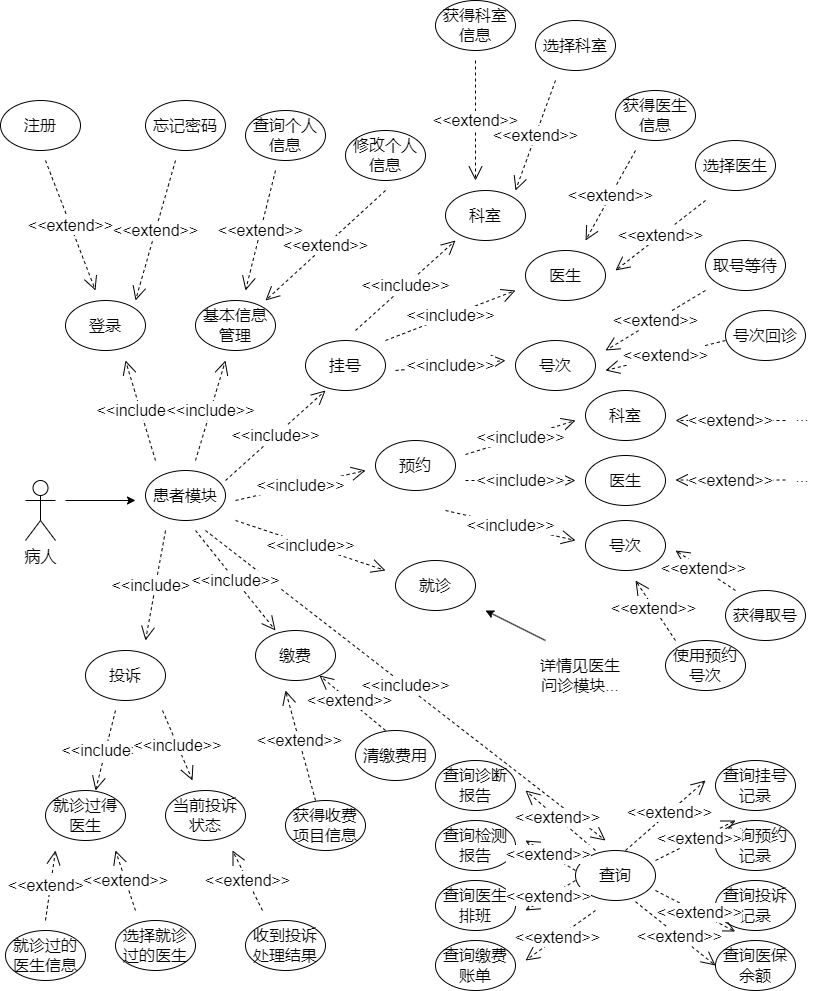
\includegraphics[width=1\textwidth]{image/example1.png}
    \caption*{图6.用例图(1)}
\end{figure}
病人端的总用例图。
\begin{figure}[H]
    \centering
    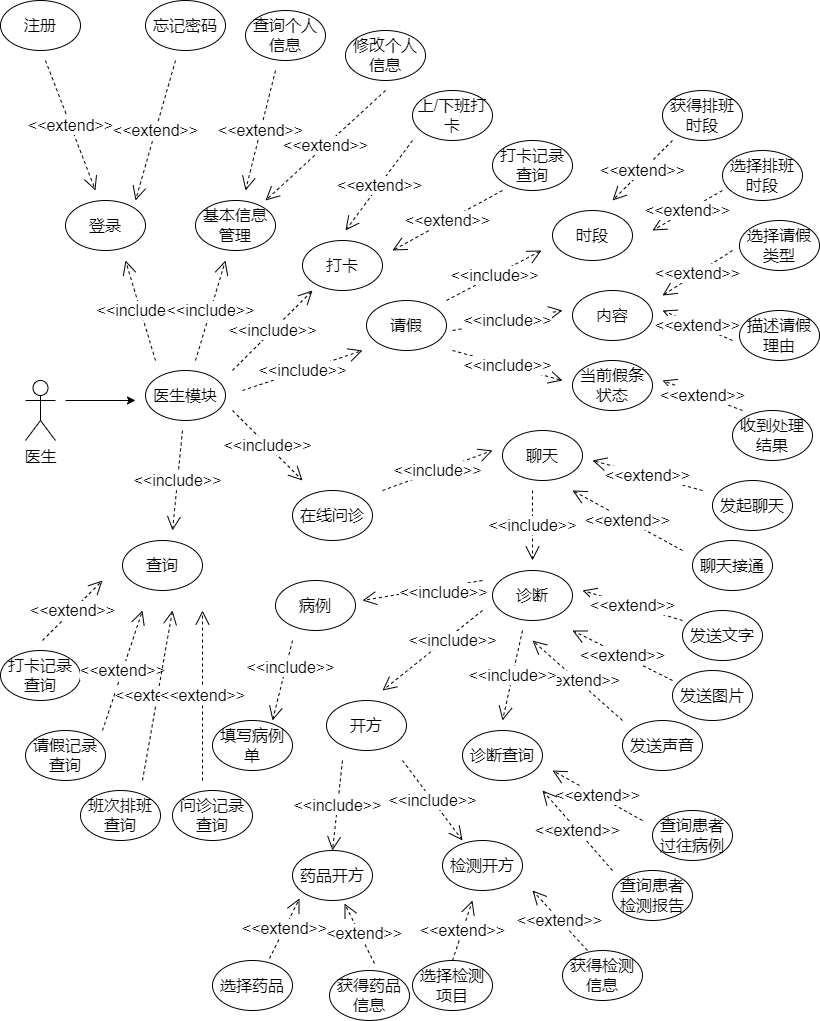
\includegraphics[width=1\textwidth]{image/example2.png}
    \caption*{图7.用例图(2)}
\end{figure}
医生端的总用例图。
\begin{figure}[H]
    \centering
    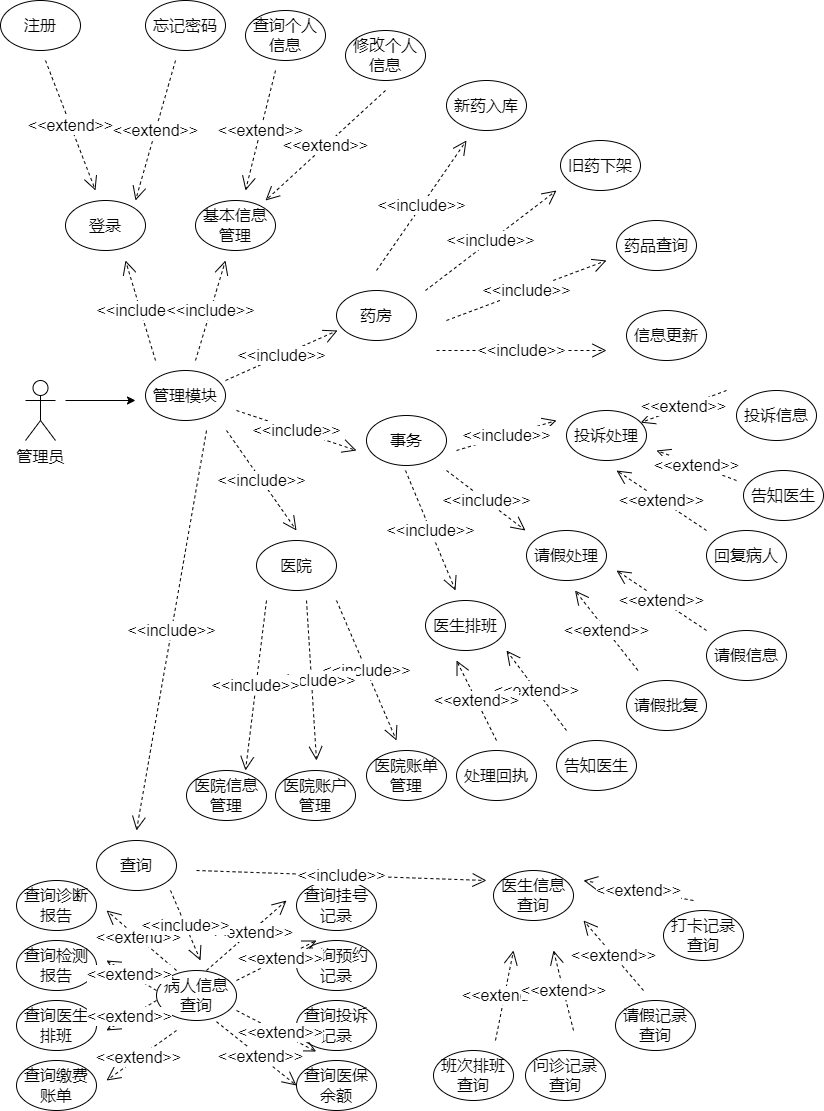
\includegraphics[width=1\textwidth]{image/example3.png}
    \caption*{图8.用例图(3)}
\end{figure}
管理端的总用例图。
\begin{figure}[H]
    \centering
    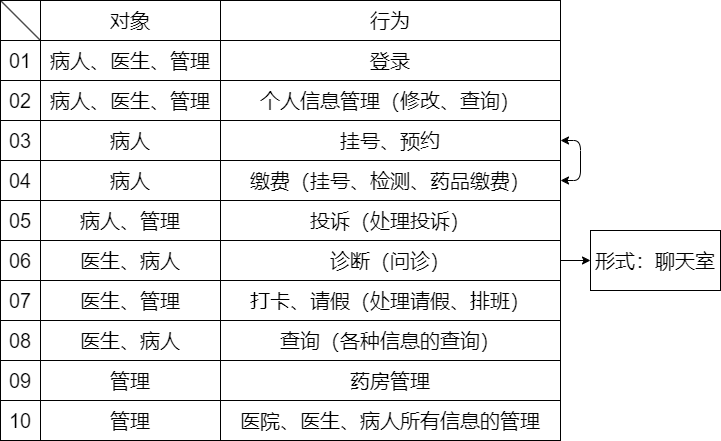
\includegraphics[width=1\textwidth]{image/collaborate.png}
    \caption*{图9.分工图}
\end{figure}
将上面的总体架构图、E-R图和用例图进行具体的细化分工之后,就得到了上面的这张分工图。分工图将整个系统分成具体的10个功能模块,其中\par
·)01、02由第二小组完成;\par
·)03、04由第一小组完成;\par
·)05、06由本小组(第三小组)完成;\par
·)07、08由第四小组完成;\par
·)09、10由第五小组完成。\par
并且每个功能模块包含\par \quad \quad(1)E-R图、(2)用例图、\par \quad \quad(3)流程图、(4)数据流图、\par \quad \quad(5)类图、(6)状态图、\par \quad \quad(7)时序图、(8)CRC卡。\par 并附上这些图片的描述和解释。
\newpage

\section*{\songti 接下来是本小组部分的图解:}
\subsection*{\songti 4.1E-R图}
\addcontentsline{toc}{subsection}{4.1E-R图}
\begin{figure}[H]
    \centering
    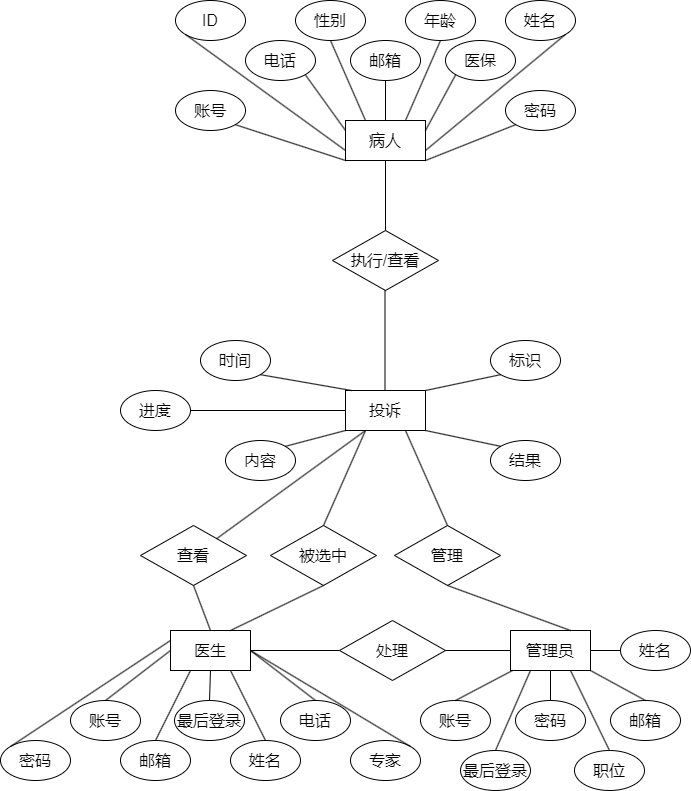
\includegraphics[width=0.5\textwidth]{images/ERGraph.png}
    \caption*{图1.E-R图示例}
\end{figure}
这是我们的ER图示例,有病人,投诉,医生,管理员等实体,以及他们之间的联系。
\subsection*{\songti 4.2用例图}
\addcontentsline{toc}{subsection}{4.2用例图}
\begin{figure}[H]
    \centering
    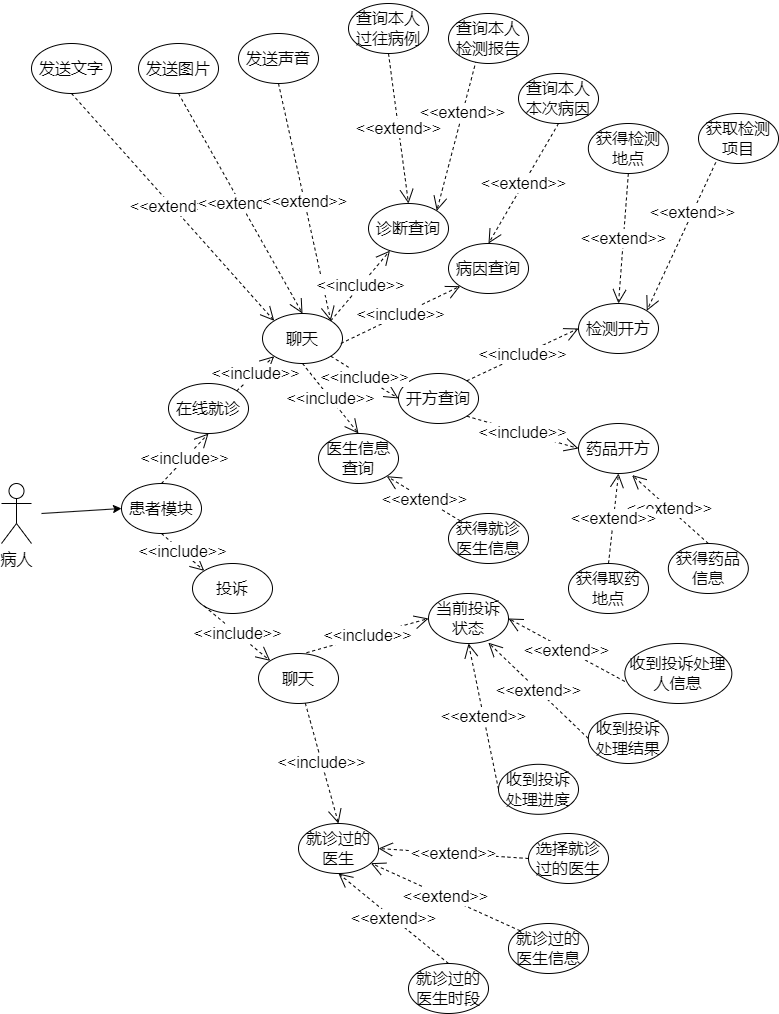
\includegraphics[width=0.75\textwidth]{images/example.png}
    \caption*{图2.用例图示例}
\end{figure}
其中,三角形箭头表示泛化关系。include箭头表示基础功能,extend箭头表示拓展功能。
\subsection*{\songti 4.3流程图}
\addcontentsline{toc}{subsection}{4.3流程图}
\begin{figure}[H]
    \centering
    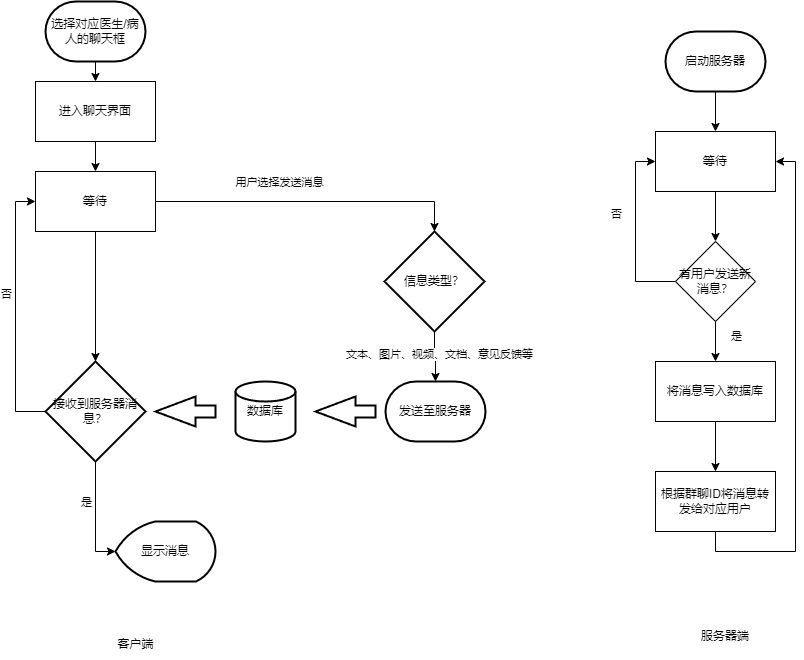
\includegraphics[width=1\textwidth]{images/pipeline.png}
    \caption*{图3.流程图示例}
\end{figure}
其中,菱形为判断分支,虚线加三边框为注解。
\subsection*{\songti 4.4数据流图}
\addcontentsline{toc}{subsection}{4.4数据流图}
\begin{figure}[H]
    \centering
    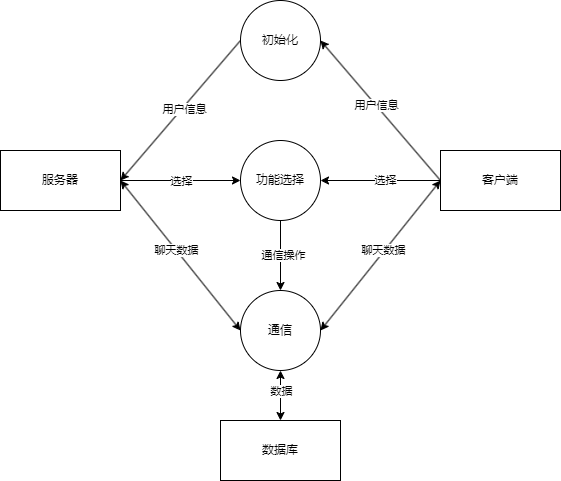
\includegraphics[width=0.75\textwidth]{images/dataStream.png}
    \caption*{图4.数据流图示例}
\end{figure}
其中,箭头代表数据流动的方向,箭头上注明数据的内容。方框代表开始和结束,圆角框代表数据处理的过程,两行则是数据存储。
\subsection*{\songti 4.5类图}
\addcontentsline{toc}{subsection}{4.5类图}
\subsubsection*{\songti 4.5.1 管理员}
\addcontentsline{toc}{subsubsection}{4.5.1 管理员}
\begin{figure}[H]
    \centering
    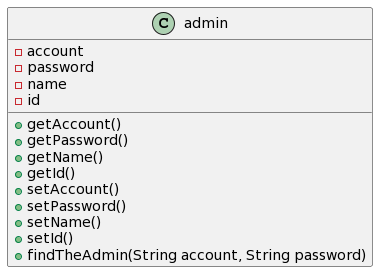
\includegraphics[width=0.75\textwidth]{images/admin.png}
    \caption*{图5.1 管理员类图示例}
\end{figure}
其中,红框代表private,绿圆代表public。
\subsubsection*{\songti 4.5.2 投诉}
\addcontentsline{toc}{subsubsection}{4.5.2 投诉}
\begin{figure}[H]
    \centering
    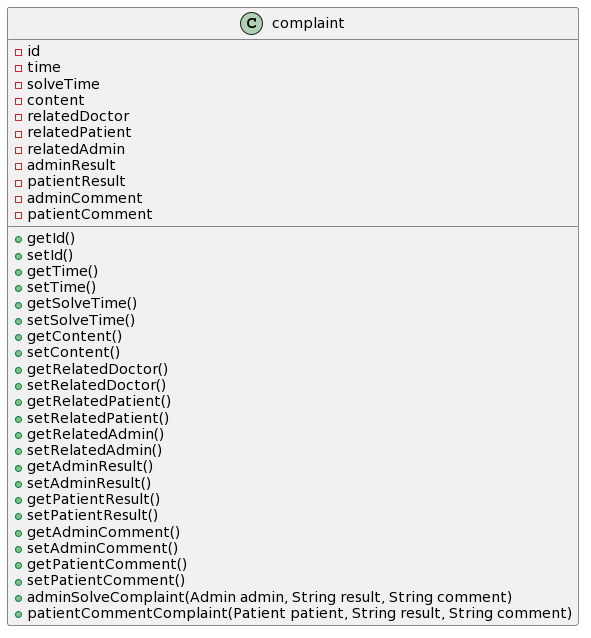
\includegraphics[width=0.75\textwidth]{images/complaint.png}
    \caption*{图5.2 投诉类图示例}
\end{figure}
其中,红框代表private,绿圆代表public。
\subsection*{\songti 4.5.3 医生}
\addcontentsline{toc}{subsubsection}{4.5.3 医生}
\begin{figure}[H]
    \centering
    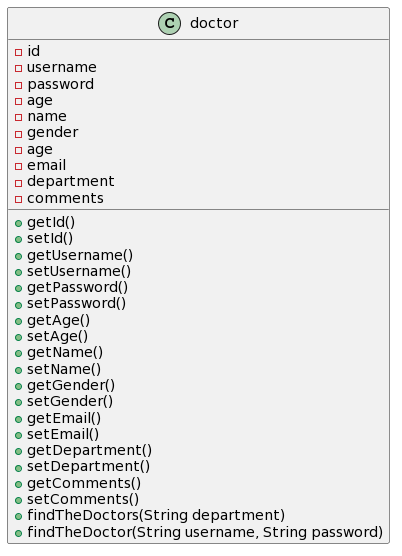
\includegraphics[width=0.75\textwidth]{images/doctor.png}
    \caption*{图5.3 医生类图示例}
\end{figure}
其中,红框代表private,绿圆代表public。
\subsection*{\songti 4.5.4 病历}
\addcontentsline{toc}{subsubsection}{4.5.4 病历}
\begin{figure}[H]
    \centering
    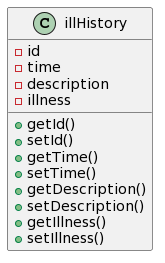
\includegraphics[width=0.75\textwidth]{images/illHistory.png}
    \caption*{图5.4 病历类图示例}
\end{figure}
其中,红框代表private,绿圆代表public。
\subsection*{\songti 4.5.5 问诊}
\addcontentsline{toc}{subsubsection}{4.5.5 问诊}
\begin{figure}[H]
    \centering
    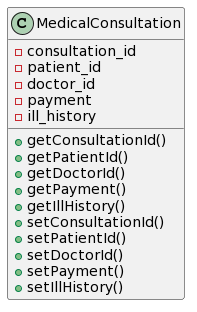
\includegraphics[width=0.75\textwidth]{images/MedicalConsultation.png}
    \caption*{图5.5 问诊类图示例}
\end{figure}
其中,红框代表private,绿圆代表public。
\subsection*{\songti 4.5.6 消息}
\addcontentsline{toc}{subsubsection}{4.5.6 消息}
\begin{figure}[H]
    \centering
    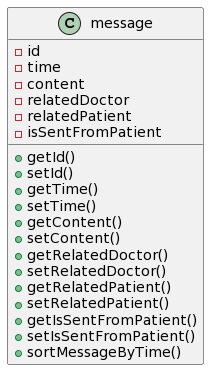
\includegraphics[width=0.75\textwidth]{images/message.png}
    \caption*{图5.6 消息类图示例}
\end{figure}
其中,红框代表private,绿圆代表public。
\subsection*{\songti 4.5.7 病人}
\addcontentsline{toc}{subsubsection}{4.5.7 病人}
\begin{figure}[H]
    \centering
    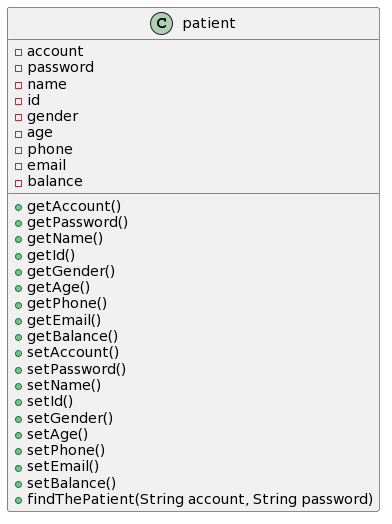
\includegraphics[width=0.75\textwidth]{images/patient.png}
    \caption*{图5.7 病人类图示例}
\end{figure}
其中,红框代表private,绿圆代表public。
\subsection*{\songti 4.6状态图}
\addcontentsline{toc}{subsection}{4.6状态图}
\begin{figure}[H]
    \centering
    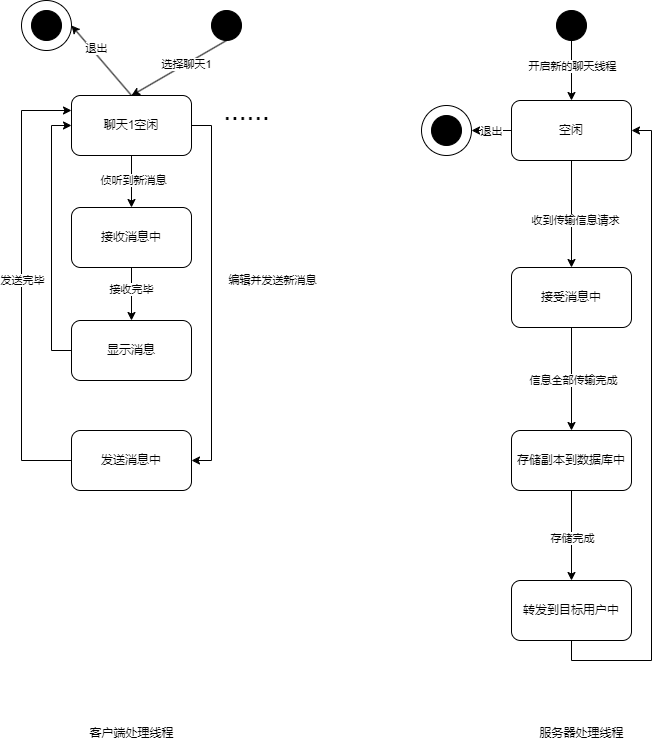
\includegraphics[width=1\textwidth]{images/state.png}
    \caption*{图7.状态图示例}
\end{figure}
其中,大圆点为开始,外面加一个环为结束。
\subsection*{\songti 4.7时序图}
\addcontentsline{toc}{subsection}{4.7时序图}
\begin{figure}[H]
    \centering
    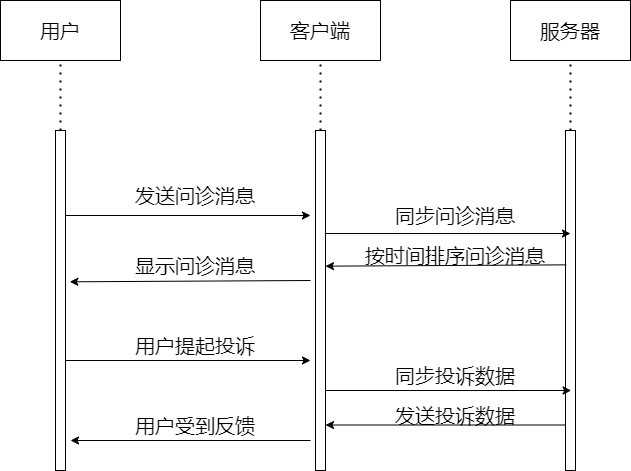
\includegraphics[width=1\textwidth]{images/time.png}
    \caption*{图7.顺序图示例}
\end{figure}
其中,竖着的圆柱条代表生命线。
\subsection*{\songti 4.8\ CRC卡}
\addcontentsline{toc}{subsection}{4.8\ CRC卡}
\begin{figure}[H]
    \centering
    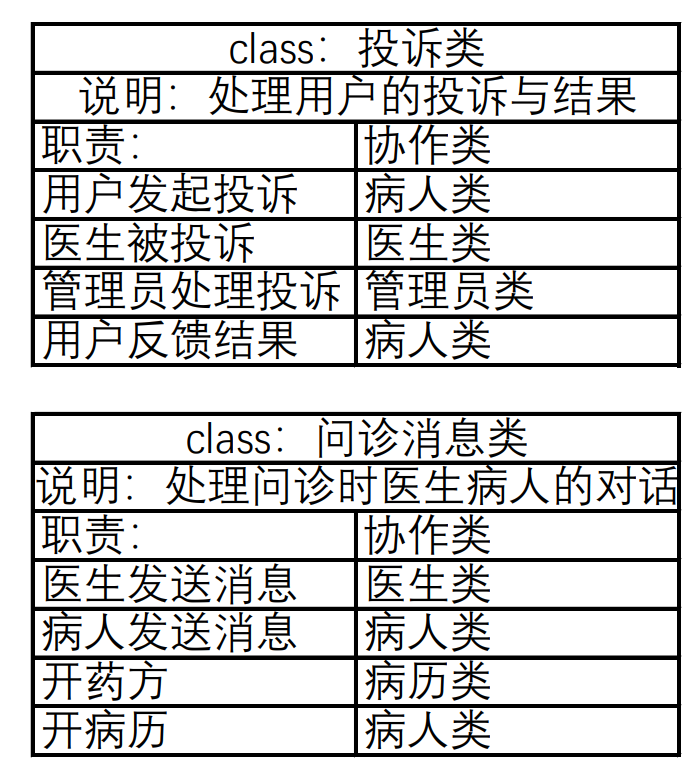
\includegraphics[width=0.5\textwidth]{images/CRCCard.png}
    \caption*{图8.CRC卡示例}
\end{figure}
\newpage

\section*{\songti 第五部分:运行环境}
\addcontentsline{toc}{section}{5.运行环境}
\subsection*{\songti 5.1服务端软硬件配置需求}
\addcontentsline{toc}{subsection}{5.1服务端软硬件配置需求}
\noindent 硬件配置:\par
1.至少1核CPU,使用Intel Xeon或类似的服务器级处理器。\par
2.内存至少4GB,以支持并发请求和数据库操作。\par
3.存储:至少50GB的高速固态硬盘(SSD),以确保快速的数据读写操作。\par
\noindent  软件配置:\par
1.操作系统:Linux(例如Ubuntu Server、CentOS)或类Unix系统,具有稳定性和安全性。\par
2.数据库:使用高性能的关系型数据库,MySQL以存储用户数据、医疗记录和系统配置。\par
3.后端框架:选择Spring Boot作为开发团队的后端框架。\par
4.Web服务器:选择Apache Tocmat服务器,用于处理HTTP请求并提供静态文件服务。\par
5.安全性:有适当的安全措施,包括防火墙、数据备份和恢复机制等。
\subsection*{\songti 5.2客户端软硬件配置需求}
\addcontentsline{toc}{subsection}{5.2客户端软硬件配置需求}
\noindent 硬件配置:\par
PC端:建议使用具有至少4GB RAM和双核CPU的计算机,以保证流畅的系统运行。\par
移动端(暂定):支持iOS和Android平台的智能手机和平板电脑,具有足够的处理能力和内存,以便用户能够顺畅地使用您的移动应用。\par
\noindent 软件配置:\par
操作系统:PC端可以支持Windows、macOS或Linux操作系统;移动端需要iOS 10或更新版本,或者Android 5.0或更新版本。\par
浏览器:对于Web应用程序,支持常见的现代浏览器,包括Chrome、Firefox、Safari和Edge等主流浏览器版本。
\newpage
\subsection*{\songti 5.3需求变更规范}
\addcontentsline{toc}{subsection}{5.3需求变更规范}
\noindent (1)提出需求变更:\par
·)用户或相关利益相关者应以书面形式提出需求变更请求,明确描述变更内容和理由。\par
·)变更请求应提交给指定的变更管理团队或项目经理。\par
\noindent (2)评估变更影响:\par
·)变更管理团队应及时评估变更对项目进度、成本和资源的影响,并与相关者讨论确认。\par
·)评估还应考虑变更对系统功能、质量和安全性的影响。\par
\noindent (3)变更批准:\par
·)只有经过适当的评估和审批后,变更才能被批准。\par
·)变更批准通常由项目管理委员会或项目经理负责。\par
\noindent (4)实施变更:\par
·)一旦变更被批准,变更管理团队应与开发团队协作,确保变更被正确实施。\par
·)变更实施后,需要进行必要的测试和验证,以确保系统功能的正确性和稳定性。\par
\subsection*{\songti 5.4故障处理规范}
\addcontentsline{toc}{subsection}{5.4故障处理规范}
\noindent (1)故障报告:\par
·)用户或系统监控应用程序应能够报告系统故障或异常。\par
·)故障报告应包括故障描述、发生时间、影响范围等相关信息。\par
\noindent (2)故障诊断:\par
·)技术支持团队应及时响应故障报告,并进行故障诊断。\par
·)诊断过程可能涉及查看日志、分析系统状态和运行情况等。\par
\noindent (3)故障修复:\par
·)一旦确定故障原因,技术支持团队应立即采取措施修复故障。\par
·)修复措施可能包括修复软件漏洞、恢复数据库、重启服务等。\par
\noindent (4)故障通知:\par
·)在故障修复过程中,相关团队应及时向用户和利益相关者通知故障进展和预计的恢复时间。\par
·)如果需要,可以提供临时解决方案或工作回退计划。\par
\noindent (5)故障跟踪与记录:\par
·)所有故障修复过程应详细记录,包括故障描述、诊断过程、修复措施和恢复时间等信息。\par
·)这些记录可以用于后续的故障分析和改进。\par
\newpage

\section*{\songti 第六部分:总结}
\addcontentsline{toc}{section}{6.总结}
\subsection*{\songti (1)充分沟通与理解:}
充分沟通与理解:在进行需求分析之前,与项目相关者进行充分的沟通和理解是至关重要的。只有通过深入了解他们的需求、期望和挑战,才能确保系统设计和开发的有效性和可行性。
\subsection*{\songti (2)明确需求优先级:}
在识别和记录需求时,要对其优先级进行明确标注。这有助于确保团队在有限的资源下优先处理最重要和最紧急的需求,同时在后续迭代中逐步完善系统。
\subsection*{\songti (3)持续迭代与反馈:}
需求分析不是一次性的任务,而是一个持续的过程。随着项目的进行和用户反馈的积累,需求可能会发生变化和调整。因此,团队应该持续进行需求的迭代和优化,并及时调整开发计划和目标。
\subsection*{\songti (4)团队合作与协调:}
需求分析是一个涉及多方利益相关者的复杂过程,需要团队成员之间的紧密合作和协调。团队应该建立良好的沟通机制和工作流程,确保信息畅通和决策高效。
\subsection*{\songti (5)文档化与记录:}
在进行需求分析时,要及时记录和文档化所有的信息和决策。这不仅有助于团队成员之间的沟通和协作,还可以作为项目后续阶段的参考和依据。
\subsection*{\songti (6)用户体验至上:}
在需求分析过程中,要始终以用户为中心,关注用户的体验和需求。通过深入理解用户的行为模式、偏好和痛点,可以设计出更符合用户期待的系统,从而提高用户满意度和系统使用率。
\subsection*{\songti (·)总的来说:}
需求分析是项目成功的关键一步,它直接影响到后续的系统设计、开发和实施。因此,团队应该认真对待需求分析工作,注重细节、沟通和持续改进,以确保项目顺利推进并达到预期目标。
\newpage
\end{document}% 结束文档编辑,后面写啥都编译不出来

%%%%%%%%%%%%%%%%%%%%%草稿%%%%%%%%%%%%%%%%%%%%%
% 插入图片 %
\begin{figure}[H]
    \centering
    \includegraphics[width=1\textwidth]{images/*.png}
    \caption*{图*.键入标题...}
\end{figure}
%%%%%%%%%%%%%%%%%%%%%%%%%%%%%%%%%%%%%%%%%%%%%